\chapter{Results and Discussion}
\label{ch:results}



\section{Results}

The results of the study indicate that the deep learning model achieved remarkable performance in classifying fake and real news articles. The model, trained on a dataset of news articles with Word2Vec embeddings, demonstrated an accuracy of nearly 99\% on the test dataset. This high accuracy suggests that the model was effective in distinguishing between fake and real news.

Furthermore, the precision, recall, and F1-score metrics for both classes (fake and real news) were consistently high, indicating the robustness of the model's performance. The precision measures the proportion of true positive predictions among all positive predictions, while recall measures the proportion of true positive predictions among all actual positive instances. The F1-score, which is the harmonic mean of precision and recall, provides a balanced assessment of the model's performance.

\begin{table}[h]
\centering
\caption{Classification report}
\label{tab:classification_report}
\begin{tabular}{lrrrr}
\toprule
& Precision & Recall & F1-score & Support \\
\midrule
0 & 0.991244 & 0.991953 & 0.991598 & 5592.000000 \\
1 & 0.991775 & 0.991050 & 0.991412 & 5475.000000 \\
Accuracy & 0.991506 & 0.991506 & 0.991506 & 0.991506 \\
Macro Avg & 0.991509 & 0.991502 & 0.991505 & 11067.000000 \\
Weighted Avg & 0.991506 & 0.991506 & 0.991506 & 11067.000000 \\
\bottomrule
\end{tabular}
\end{table}

\begin{figure}
    \centering
    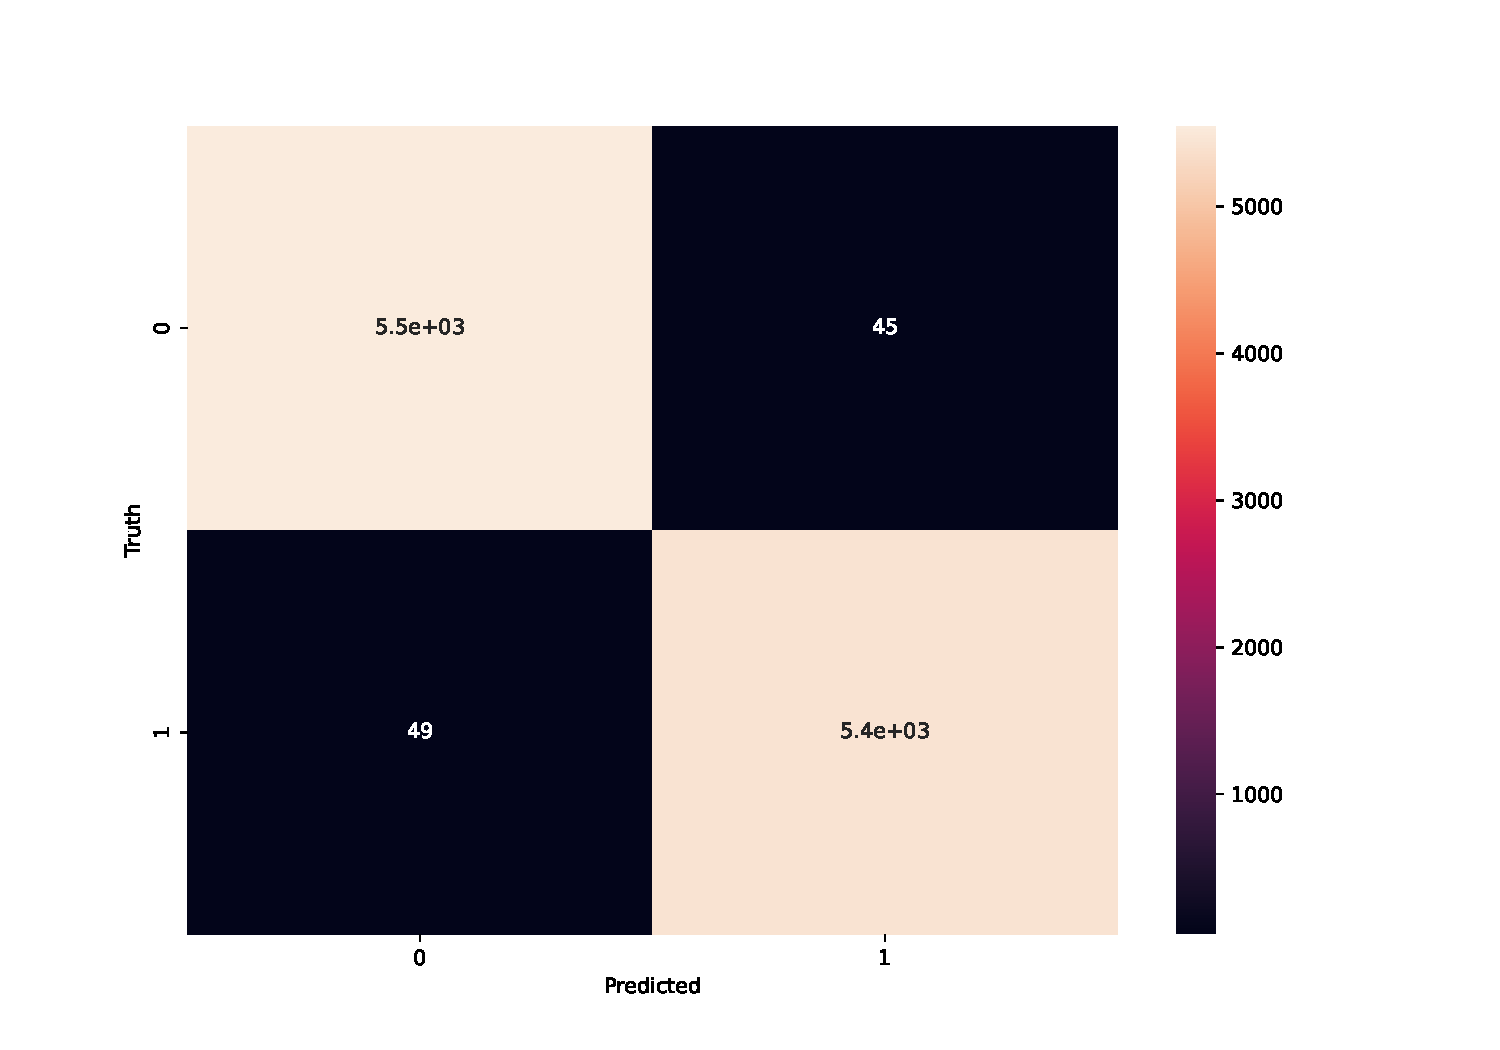
\includegraphics[width=0.75\linewidth]{figures/confusion_matrix.pdf}
    \caption{confusion matrix}
    \label{fig:enter-label}
\end{figure}

\section{Discussion}

The impressive performance of the deep learning model can be attributed to several factors. Firstly, the utilization of Word2Vec embeddings enabled the model to capture semantic and syntactic similarities between words, enhancing its understanding of the textual data. This embedding technique facilitated the representation of words as dense vectors in a continuous vector space, enabling the model to learn meaningful representations of words based on their context.

Additionally, the use of a Long Short-Term Memory (LSTM) neural network architecture proved effective in capturing long-range dependencies in the sequential data. LSTMs are well-suited for processing sequential data, such as text, as they can retain information over extended sequences and mitigate the vanishing gradient problem often encountered in deep learning models.

The model's ability to accurately classify fake and real news articles has significant implications for combating misinformation and disinformation in online media. By automatically identifying and flagging potentially misleading content, the model can assist journalists, fact-checkers, and social media platforms in curbing the spread of false information and promoting media literacy among the public.

\section{Analysis}

The analysis of the model's performance highlights its effectiveness in addressing the challenge of fake news detection. The high accuracy, precision, recall, and F1-score metrics demonstrate the model's capability to reliably identify fake news articles while minimizing false positives and false negatives.

Moreover, the deployment of the model in real-world settings could have profound implications for mitigating the societal impact of misinformation. By integrating the model into news aggregation platforms, social media networks, and content moderation systems, stakeholders can leverage AI-powered solutions to safeguard users from consuming misleading or harmful content.

However, it is essential to acknowledge the limitations and challenges associated with AI-based approaches to fake news detection. These include issues related to bias, fairness, privacy, and the arms race between misinformation creators and detection systems. Addressing these challenges requires interdisciplinary collaboration and ongoing research efforts to develop robust, ethical, and transparent solutions.

Overall, the results and analysis presented in this study underscore the potential of deep learning models in combating misinformation and promoting media integrity in the digital age. By harnessing the power of AI, researchers and practitioners can contribute to building a more informed, resilient, and trustworthy information ecosystem.


\section{Limitations}

Despite the promising results, several limitations should be acknowledged in this study. Firstly, the model's performance may be influenced by the quality and representativeness of the training data. Biases or inaccuracies in the dataset could affect the model's generalization to unseen data and its ability to detect nuanced forms of misinformation.

Furthermore, the reliance on Word2Vec embeddings may restrict the model's understanding of contextual nuances and linguistic subtleties in news articles. More advanced embedding techniques, such as contextualized word embeddings or transformer-based models, could potentially enhance the model's semantic understanding and classification accuracy.

Additionally, the evaluation metrics used in this study provide a quantitative assessment of the model's performance but may not fully capture its real-world effectiveness. Factors such as the prevalence of fake news in the media landscape, the consequences of false positives and false negatives, and the dynamic nature of misinformation campaigns warrant further investigation.

\section{Summary}

In summary, this study explored the application of deep learning techniques for fake news detection, leveraging Word2Vec embeddings and LSTM neural networks. The results demonstrated the model's high accuracy and effectiveness in classifying fake and real news articles. Despite the promising findings, several limitations exist, including dataset biases, embedding constraints, and evaluation metric considerations.

Moving forward, future research should focus on addressing these limitations and advancing the state-of-the-art in fake news detection. This includes incorporating more sophisticated embedding techniques, exploring ensemble learning approaches, and conducting rigorous evaluations in diverse media environments. By overcoming these challenges, researchers and practitioners can contribute to building more robust and reliable systems for combating misinformation in the digital era.

 

 

 



